%\documentclass{article}
%\usepackage{graphicx,subfigure}
%\begin{document}

\begin{figure}[h]
  \centering
  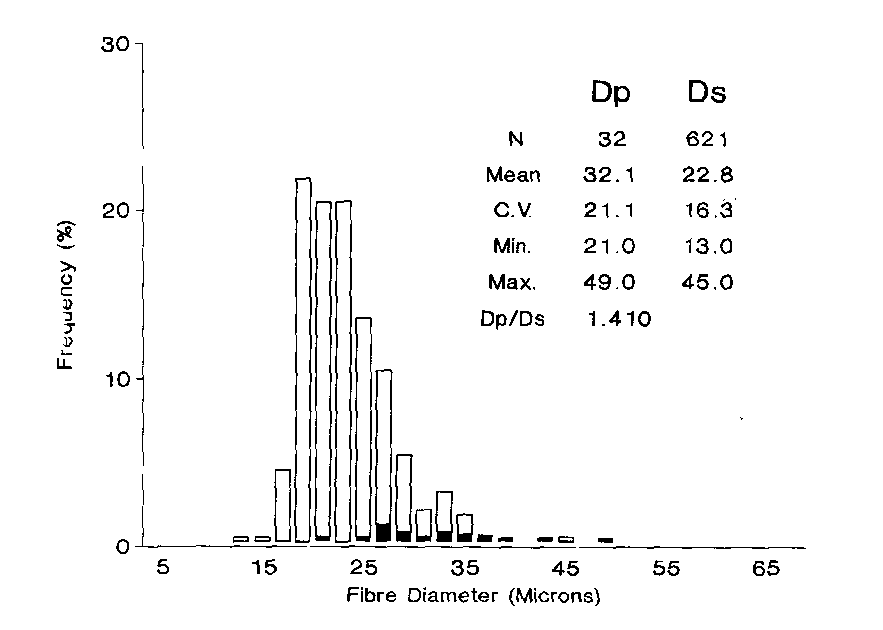
\includegraphics[width=\textwidth,trim = 0 0 0 120]{images/fig15ri.png}
  \caption{ Fibre diameter histogram of a 1976 drop hogget ewe from CSIRO
      experiment No. 1.  Note that the frequency of large primary and
      secondary fibres is not as large as in Figure~\ref{fig:13},
      but is higher than in Figure~\ref{fig:4}.}
  \label{fig:15}
\end{figure}

%\end{document}
